Computational efficiency has implications for the prediction's accuracy and the cost of deployment. Since forecasting systems are constantly retrained to address distributional shifts, orders-of-magnitude improvements in speed can easily translate into orders-of-magnitude price differences deploying the models. This section explores the implications of computational efficiency in the accuracy gains associated with hyperparameter optimization and training economic costs.

\textbf{Hyperparameter Optimization}. Despite all the progress improving the computation efficiency of Transformer-based methods, see Figure~\ref{fig:computational_cost_comparison}, their speed and memory requirements make exploring their hyperparameter space unaffordable in practice, considering the amount of GPU computation they still require. % The diminishing returns nature of the exploration gains makes this problem even more pronounced. 

\begin{figure}[!ht]
\centering
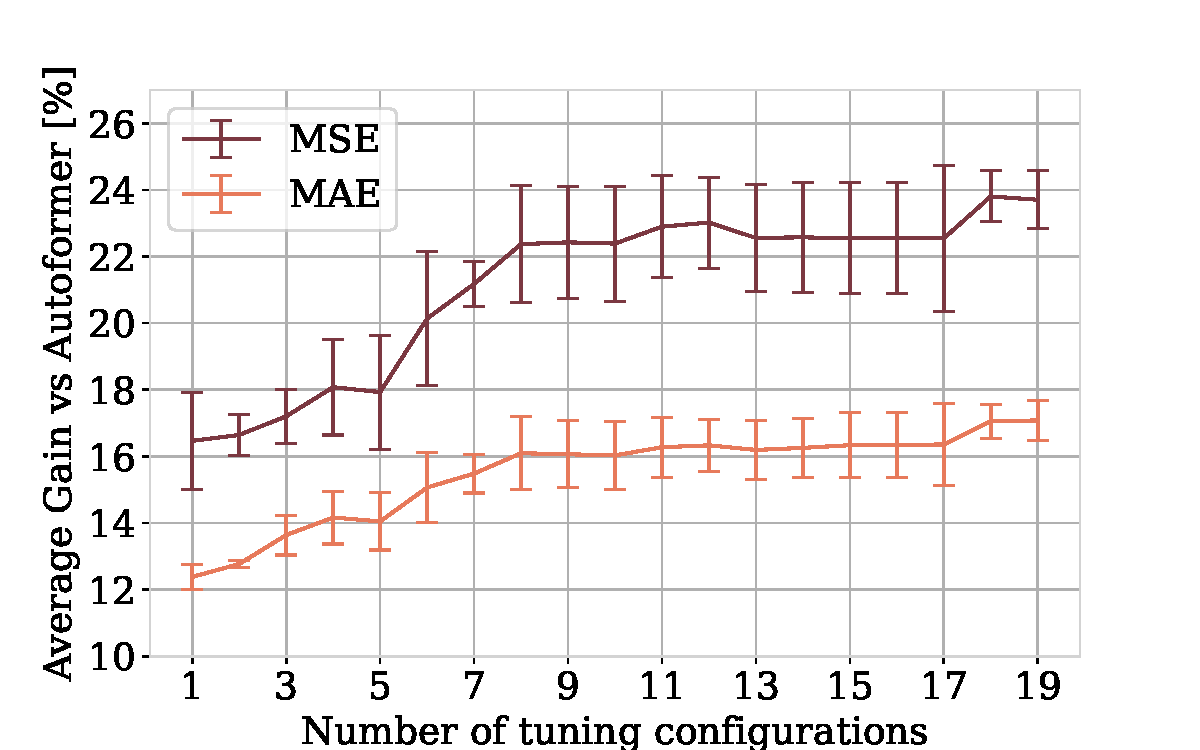
\includegraphics[width=0.8\linewidth]{images/gain_vs_grid.pdf}
\caption{\ours\ performance improvement over \Autoformer\ as a function of explored hyperparameter configurations.} \label{fig:ablation_gain_grid}
\end{figure}

For this experiment we report the iterations of the \emph{hyperparameter optimization phase}, described in Section~\ref{section:training_methodology}, where we explore the hyperparameters from Table~\ref{table:hyperparameters} using \HYPEROPT, a Bayesian hyperparameter optimization library~\citep{bergstra2011hyperopt}. As shown in Figure~\ref{fig:ablation_gain_grid} the exploration exhibits monotonic relative performance gains of \ours\ versus the best reported \Autoformer~\citep{wu2021autoformer} in the ablation datasets. %\EDIT{We wonder if a more extensive hyperparameter search could alleviate the stark performance difference.}

\textbf{Training Economic Costs}. We measure the train time for \ours, \NBEATSg\ and Transformer-based models, on the six main experiment datasets and 8 runs. We rely on a AWS \model{g4dn.2xlarge}, with an NVIDIA T4 16GB GPU.

We differentiate between \ours$_{1}$, our method with a single \HYPEROPT\ iteration randomly sampled from Table~\ref{table:hyperparameters}, and \ours$_{20}$\ to our method after 20 \HYPEROPT\ iterations. For the Transformer-based models we used optimal hyperparameters as reported in their repositories. Table~\ref{table:ablation_training_time} shows the measured train time for the models, \ours$_{1}$\ takes 1.5 hours while more expensive architectures like \Autoformer\ or \Informer\ take 92.6 and 62.1 hours each. Based on hourly prices from January 2022 for the \model{g4dn.2xlarge} instance, USD 0.75, the main results of the paper would cost nearly USD 70.0 with \Autoformer, USD 46.5 with \Informer, while \ours$_{1}$\ results can be executed under USD 1.5 and \ours$_{20}$\ with USD 22.8. Figure~\ref{fig:ablation_gain_grid}, shows that \ours$_{1}$ achieves a 17\% MSE average performance gain over \Autoformer\ with 1.6\% of a single run cost, and \ours$_{20}$\ almost 25\% gain with 33\% of a single run cost. A single run does not consider hyperparameter optimization.

\begin{equation*}
    \text{ExptPrice} = \text{GPUPrice} \times \text{HyperOptIters} \times \text{TrainTime} \times \text{Runs} 
\end{equation*}

\begin{table}[!ht]
\tiny
\scriptsize
    \begin{center}
        \caption{Train time in hours on a \model{g4dn.2xlarge} instance.} 
        \label{table:ablation_training_time}
    \setlength\tabcolsep{2.3pt}
    \begin{tabular}{ll | ccccc}  \toprule
    &  Horizon    & \ours$_{1}$  & \ours$_{20}$         & \Autoformer       & \Informer         & \NBEATSg          \\ \midrule
    \parbox[t]{0.2mm}{\multirow{4}{*}{\rotatebox[origin=c]{90}{A. Time}}}
    & 96/24       & 0.183        & 3.66                 & 12.156            & 9.11              & 0.291             \\
    & 192/36      & 0.257        & 5.14                 & 16.734            & 11.598            & 0.462             \\
    & 336/48      & 0.398        & 7.96                 & 22.73             & 15.237            & 0.674             \\
    & 720/60      & 0.682        & 13.64                & 40.987            & 26.173            & 1.249             \\ \midrule
    & Total       & 1.523        & 30.46                & 92.607            & 62.118            & 2.676             \\ \bottomrule
    \end{tabular}
    \end{center}
\end{table}
